\documentclass[conference]{IEEEtran}
\IEEEoverridecommandlockouts
% The preceding line is only needed to identify funding in the first footnote. If that is unneeded, please comment it out.
\usepackage{cite}
\usepackage{amsmath,amssymb,amsfonts}
\usepackage{algorithmic}
\usepackage{graphicx}
\usepackage{textcomp}
\usepackage{xcolor}
\usepackage{hyperref}
\usepackage{seqsplit}
\def\BibTeX{{\rm B\kern-.05em{\sc i\kern-.025em b}\kern-.08em
    T\kern-.1667em\lower.7ex\hbox{E}\kern-.125emX}}
\begin{document}

\title{CPEN 442 Project Proposal}

\author{\IEEEauthorblockN{Mike Yue, Student Number: 24583156}
\IEEEauthorblockN{Ben Henaghan, Student Number: 96671466}
\IEEEauthorblockN{Austine Yapp Student Number: TODO}
\IEEEauthorblockN{Scott Wang, Student Number: 72573322}}

\maketitle

\textbf{\textcolor{red}{REMEMBER TO WRITE IN PAST TENSE}}

\begin{abstract}
	This project addressed the issue of keypad locks being highly vulnerable to a variety of simple attacks by implementing an internet conected keypad which utilised one-time passcodes. This retained the usefulness of a keypad (as opposed to a key lock) while greatly increasing security.
\end{abstract}

\section{Introduction}
	Keypad door locks are increasingly being used in society today, with many more commercial homes and even industrial factories switching from traditional key locks to keyless keypad door locks. Although the advent of such locks provides users with the much-desired convenience of keyless entry/exit, it is still relatively vulnerable as a security layer in preventing adversarial break-ins into seemingly secure compounds. 

\begin{figure}[htbp]
\centerline{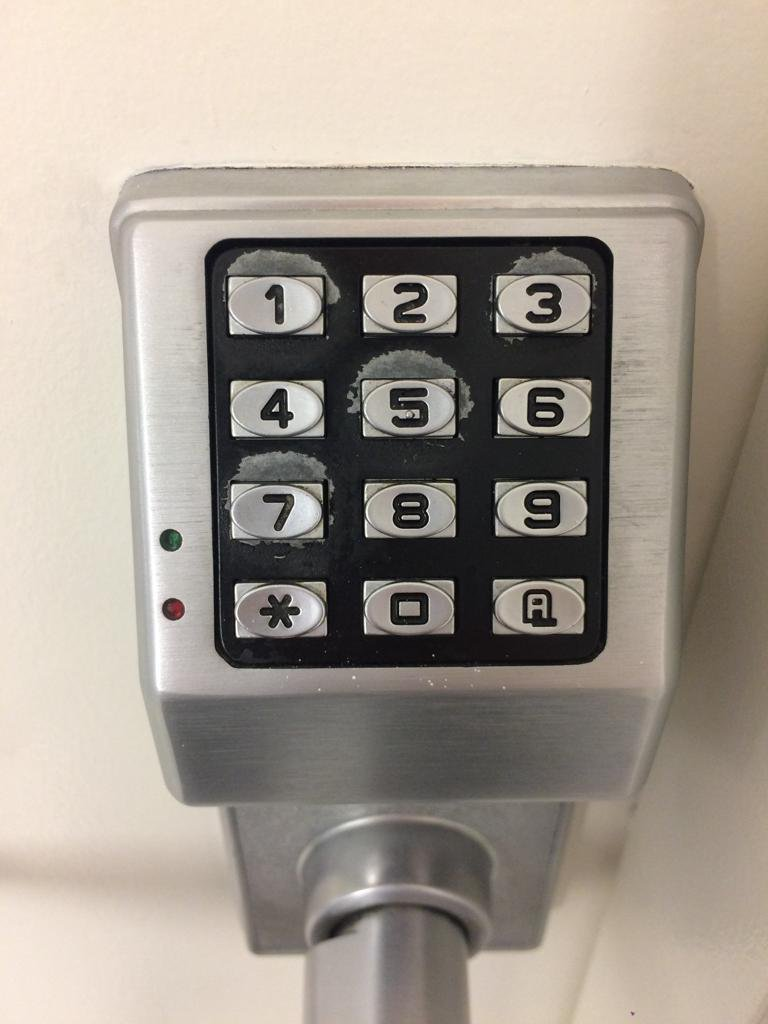
\includegraphics[width=0.5\textwidth]{worn_lock.jpg}}
\caption{A Keypad lock where button wear gives away the digits used in the code.}
\label{fig:worn_lock}
\end{figure}

Upon further inspection, the vulnerabilities of a keypad door lock become increasingly apparent. 

One such vulnerability that the keypad door lock inherently possesses is  the susceptibility of wear after prolonged use. Mechanical wear through direct and erosive contact with the keypad, as well as chemical wear through reactions with natural skin-oils may cause keypad door locks to quickly show signs of fatigue. In Figure 1, the keypad numbers 1, 3, 5 and 7 are clearly worn out compared to the others. An adversary would thus only require a total of 4! = 24 permutations of access codes in order to crack the users’ access code.

Furthermore, the repetitive use of the static access codes may be vulnerable to shoulder surfing/pinhole camera recording attacks from adversaries. An adversary simply needs to identify the users’ static access code in order to have full access to the compounds. One relatively easy method would be to simply install a pinhole camera in an inconspicuous position over the keypad door lock. With any unobstructed video capture of a users’ entry, adversaries may quickly figure out the access code for that lock.
This project thus strives to introduce additional layers of security through the use of dynamically-generated One Time Access codes. Given the keypad door locks’ extensive use in both commercial and industrial markets, the value of the assets that are secured by it is practically priceless, seeing as it protects most users’ households. Such a security analysis of the system is therefore of paramount importance, seeing as its vulnerabilities pose a threat to the incalculable worth of the users’ assets. 

\section{Current Solutions}
For security purposes, most keypad door locks in the market allow users to reset their door code. And periodic code change is encouraged in case the adversary steals the previous code. However, there is typically no restriction on how often keypad codes can be changed, which increases the vulnerability of the keypad door locks significantly.
Therefore, users need to manually reset their door code on a regular basis to ensure the security of the entry to their houses, which is the redundant and tiresome task for most people.

\section{Our Implementation}
The project focuses on the security improvement of a specific subset of digital locks, Smart locks, locks which can connect to remote servers.

Each user possesses their own individual entry code which changes every time it’s used, as well as a unique identification code that remains static. To gain access, the user enters their identification code followed by their entry code. The lock securely transmits the entered credentials to the server, and the server validates the request based on the credentials and entry code. If the server approves the request, it does three things. It sends an acknowledgement to the smart lock for it to grant entry, it generates a new random entry code, and it sends the new entry code to the user via email. 

By replacing the entry code every time it has been used to successfully enter the house, pinhole camera/shoulder surfing recording attacks become next to useless, as the code they record will become useless the instant it’s used. Furthermore,
\section{Comparison to Competitng Solutions}

\section{Plan for Project}
\subsection{Hardware Development}
	Our project required a prototype hardware system on which to test the software. This meant that it was imperitive to have a functioning hardware component as early in the development cycle as possible. The project team agreed to finalise a design for the prototype hardware by October 25\textsuperscript{th} in order to give sufficient lead time to order compoonents and build the hardware by November 8\textsuperscript{th}.


	This finalisation of the prototype hardware did not signal the end of hardware development for the project, we decided to keep developing the physical lock system to make it a more compelling commercial product.

\subsection{Software Developement}
	Software development started with the establishment of a strict protocol between the client and server for authentication and sending the user their one-time key. Concurrently, the broad OOP software design for the server and client android application was defined.

	After the software design was completed (which was planned to be finalized by November 1\textsuperscript{st}) full software development was started. We chose to adopt an agile-like methodology where developement was broken up into 1 week `sprints' with key tasks for each team member to complete.

\subsection{Development and Testing Methodology}
	We chose to make use of `Test Driven Design' as a core part of our software development process. Unit testing was used for most back-end software and integration/system tests were created for critical or complex components.

	Hardware testing comprised mostly of testing the functionality of our prototype --- security testing of the prototype hardware was avoided as we felt it was less relevant to our prototype and would incurr extra materials cost if any destructive testing was undertaken.



\end{document}
